\section{Untersuchung der Kinematik}
Der erste Schritt besteht darin die kinematischen Zusammenhänge des Systems zu analysieren. Im Fall, dass der Würfel auf einer Kante balanciert, verfügt dieser über zwei rotatorische Freiheitsgrade, von denen der erste durch die generalisierte Koordinate $\varphi$ beschrieben wird und die Orientierung des Würfelgehäuses wiedergibt. Die zweite generalisierte Koordinate $\psi$ erfasst die Rotation der Schwungmasse relativ zu dem Würfelgehäuse.
\begin{figure}[!ht]
\centering
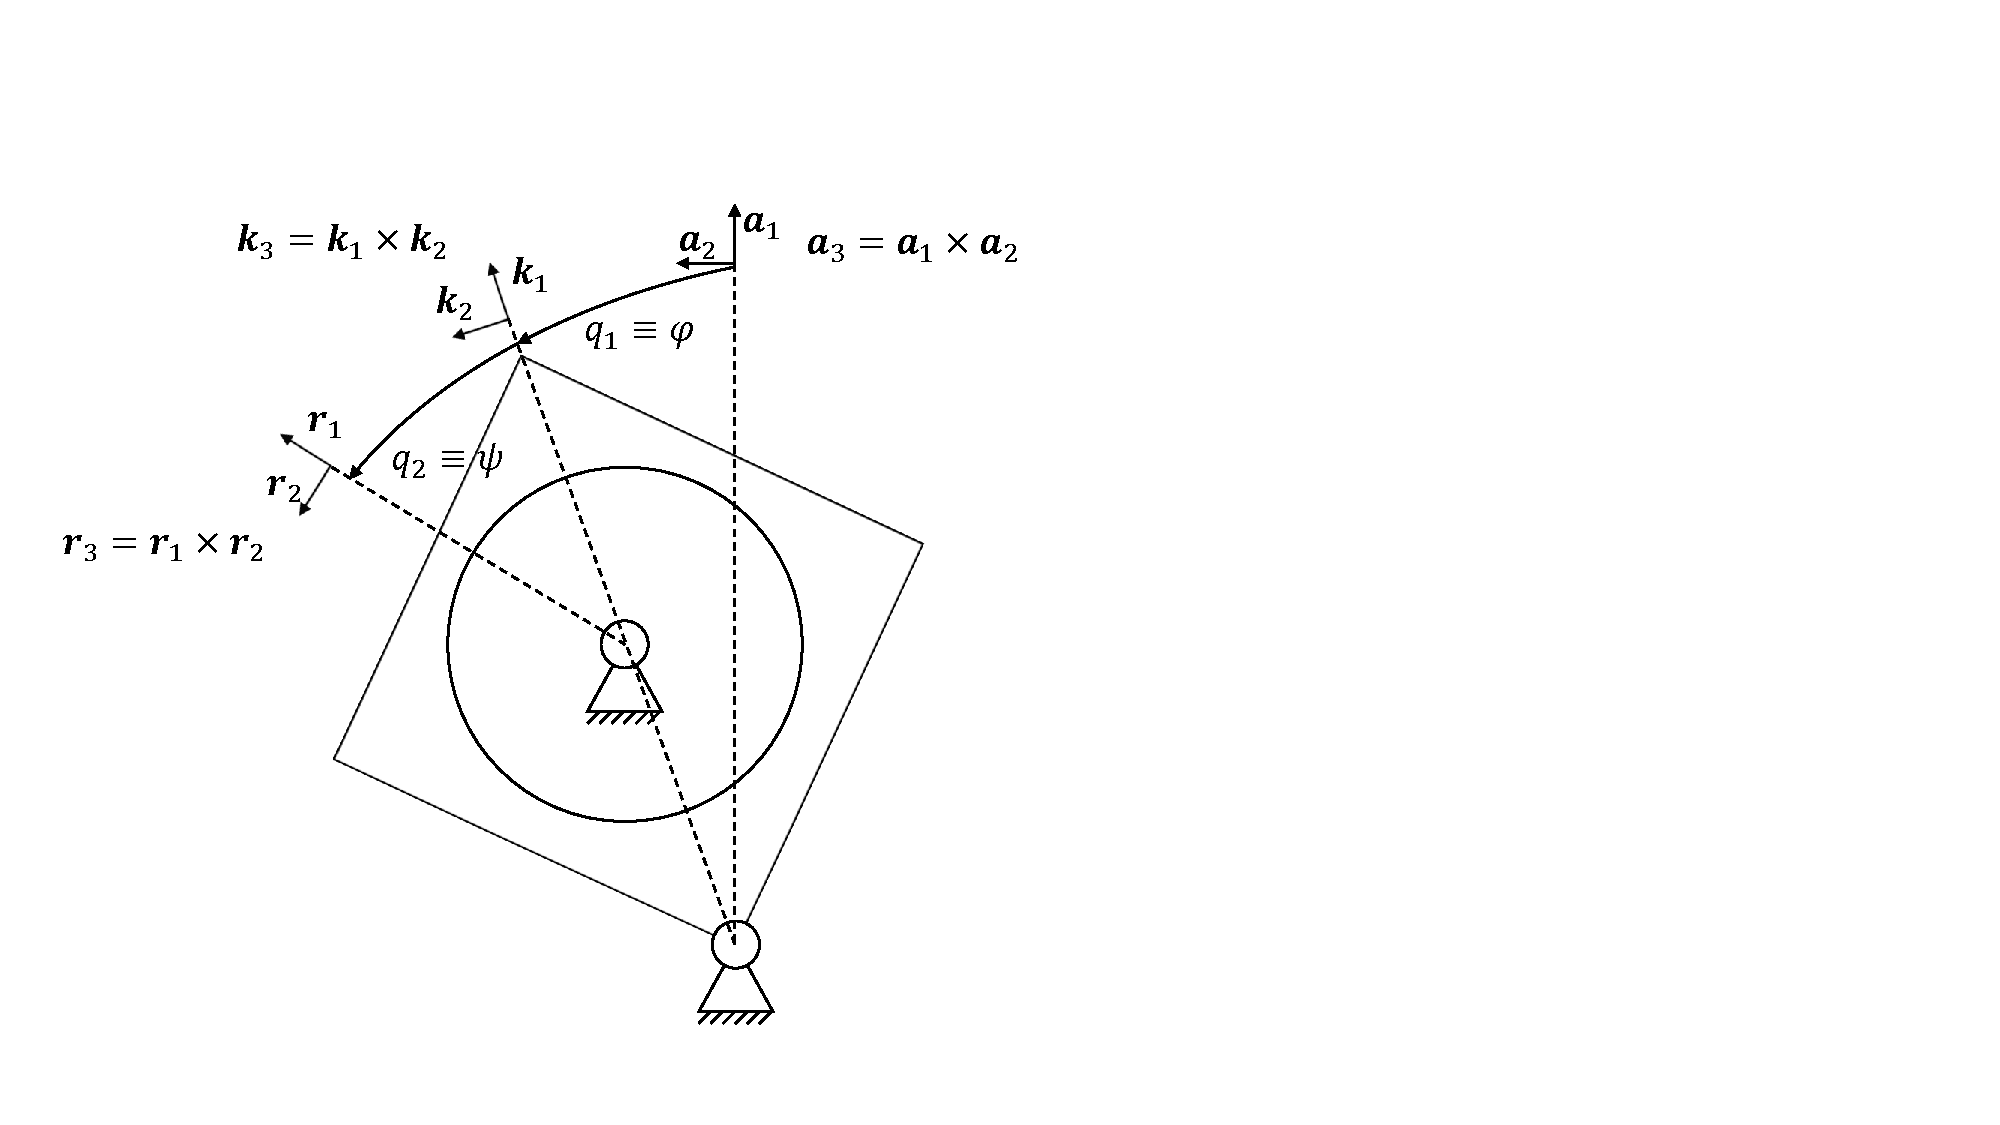
\includegraphics[width=0.6\linewidth, trim={1cm 1.5cm 18cm 3.5cm}, clip]{img/ModellWuerfelseite}
\caption{Kinematikplan des Würfels auf einer Kante}
\label{skizze_dynamik_edge}
\end{figure}

Um die Körper des Systems zu modellieren werden im nächsten Schritt die Bezugssysteme $A$, $K$ und $R$ eingeführt, wobei ein beliebiges Bezugssystem $B$ durch drei Vektoren $\bs{b_i} \ i \in \{1,2,3\}$ definiert wird. Die Vektoren $\bs{b_i}$ werden als Vektorbasis bezeichnet.\footnote{Allgemein genügen drei linear unabhängige Vektoren als Vektorbasis, allerdings werden in dieser Arbeit ausschließlich paarweise orthogonale Einheitsvektoren verwendet, da diese eine einfachere Handhabung ermöglichen. Im weiteren Verlauf wird nicht explizit erwähnt, dass es sich bei den Vektorbasen um paarweise orthogonale Einheitsvektoren handelt.} In diesem Fall ist $A$ ein Intertialsystem, das heißt die Ausrichtung der Vektoren $\bs{a_i}$ ist konstant. Deshalb wird $A$ bzw. dessen Vektorbasis auch als raumfest bezeichnet. Bei $K$ handelt es sich um ein körperfestes Bezugssystem, die Vektoren $\bs{k_i}$ sind an dem Würfelgehäuse fixiert und ändern ihre Ausrichtung in Abhängigkeit von $\varphi$. Das Bezugssystem $R$ ist ebenfalls körperfest, wobei die Vektorbasis an der Schwungmasse fixiert ist. Folglich beschreiben die Koordinaten $\varphi$ und $\psi$ die Rotation von $K$ relativ zu $A$ bzw. von $R$ gegenüber $K$. 

Mittels eines Bezugssystems kann ein beliebiger Vektor als Linearkombination der Vektorbasis dargestellt werden. Als Beispiel sei der Ortsvektor $\bs{c}$ des Würfelschwerpunktes genannt, wobei das verwendete Bezugssystem durch die vorangehenden Hochstellung gekennzeichnet wird.
\begin{equation}
\bs{c} = l\idx{C} \cdot \bs{k}\idx{1} + 0 \cdot \bs{k}\idx{2} + 0 \cdot \bs{k}\idx{3} = \vecBS{K}{l\idx{C}}{0}{0}
\end{equation}
Um nun die Komponenten $\alpha_i$ des Vektors $\bs{c}$ in dem Bezugssystem $A$ zu erhalten, muss das Skalarprodukt $\inProd{\bs{a}_i}{\bs{c}}$ berechnet werden. Wird dieser Ansatz auf alle drei Komponenten appliziert ergibt sich der Zusammenhang\footnote{Um die allgemeine Gültigkeit der linearen Abbildung zu verdeutlichen wird in dieser Gleichung die Definition $\bs{c}=\vecBS{K}{l_C}{0}{0}\equiv\vecBS{K}{\beta_1}{\beta_2}{\beta_3}$ verwendet.}
\begin{equation}
\begin{split}
\bs{c} &= \vecBS{A}{\alpha\idx{1}}{\alpha\idx{2}}{\alpha\idx{3}} = \inProd{\bs{c}}{\bs{a}\idx{1}}\cdot \bs{a}\idx{1} + \inProd{\bs{c}}{\bs{a}\idx{2}}\cdot\bs{a}\idx{2} + \inProd{\bs{c}}{\bs{a}\idx{3}}\cdot\bs{a}\idx{3} 
= \vecBS{A}{\inProd{\bs{c}}{\bs{a}\idx{1}}}{\inProd{\bs{c}}{\bs{a}\idx{2}}}{\inProd{\bs{c}}{\bs{a}\idx{3}}}
\\
&= \vecBS{A}
{\beta\idx{1}\cdot\inProd{\bs{a}\idx{1}}{\bs{k}\idx{1}} + \beta\idx{2}\cdot\inProd{\bs{a}\idx{1}}{\bs{k}\idx{2}} + \beta\idx{3}\cdot\inProd{\bs{a}\idx{1}}{\bs{k}\idx{3}}}
{\beta\idx{1}\cdot\inProd{\bs{a}\idx{2}}{\bs{k}\idx{1}} + \beta\idx{2}\cdot\inProd{\bs{a}\idx{2}}{\bs{k}\idx{2}} + \beta\idx{3}\cdot\inProd{\bs{a}\idx{2}}{\bs{k}\idx{3}}}
{\beta\idx{1}\cdot\inProd{\bs{a}\idx{3}}{\bs{k}\idx{1}} + \beta\idx{2}\cdot\inProd{\bs{a}\idx{3}}{\bs{k}\idx{2}} + \beta\idx{3}\cdot\inProd{\bs{a}\idx{3}}{\bs{k}\idx{3}}}
\\
&= \presuper{K}{\begin{pmatrix}
\underbrace{
\begin{bmatrix}
\inProd{\bs{a}\idx{1}}{\bs{k}\idx{1}} & \inProd{\bs{a}\idx{1}}{\bs{k}\idx{2}} & \inProd{\bs{a}\idx{1}}{\bs{k}\idx{3}} \\
\inProd{\bs{a}\idx{2}}{\bs{k}\idx{1}} & \inProd{\bs{a}\idx{2}}{\bs{k}\idx{2}} & \inProd{\bs{a}\idx{2}}{\bs{k}\idx{3}} \\
\inProd{\bs{a}\idx{3}}{\bs{k}\idx{1}} & \inProd{\bs{a}\idx{3}}{\bs{k}\idx{2}} & \inProd{\bs{a}\idx{3}}{\bs{k}\idx{3}}
\end{bmatrix}}_{\equiv \pMat{K}{A}} \cdot \underbrace{\begin{bmatrix}
\beta\idx{1} \\ \beta\idx{2} \\ \beta\idx{3}
\end{bmatrix}}_{= \presuper{K}{\bs{c}}}
\end{pmatrix}} 
= \presuper{A}{\begin{pmatrix}
\begin{bmatrix}c_{\varphi} & -s_{\varphi} & 0 \\ s_{\varphi} & c_{\varphi} & 0 \\ 0 & 0 & 1 \end{bmatrix} \cdot \presuper{K}{\bs{c}} \end{pmatrix}}\,.
\end{split}
\end{equation}
Somit handelt es sich bei der Projektion eines Vektors, welcher in einem beliebigen Bezugssystem $A$ dargestellt ist, in ein weiteres Bezugssystem $B$ um eine lineare Abbildung. Die Abbildungsvorschrift wird durch die Matrix $\pMat{B}{B}$ definiert. Des Weiteren zeigt dieses Beispiel die perspektivische Bedeutung eines Bezugssystem. Wird der Vektor $\bs{c}$ in $K$ dargestellt, hängt er lediglich von der Länge $l_C$ ab und ist folglich konstant. Aus der Perspektive von $A$ ist der Vektor eine Funktion von $\varphi$ und somit variabel. Die Begründung hierfür liegt darin, dass das Intertialsystem $A$ die Bewegung des Würfels im Raum wahrnimmt, wodurch der Ortsvektor des Schwerpunktes variabel erscheint.
Im Gegensatz dazu erfasst das körperfeste Bezugssystem $K$ einen Vektor aus der Perspektive des Würfelkörpers, weshalb der in $K$ dargestellte Ortsvektor $\presuper{K}{\bs{c}}$ des Schwerpunktes konstant ist.
Dieser Umstand kann genutzt werden, indem ein Vektor zunächst in einer einfachen Form dargestellt und anschließend in das gewünschte Bezugssystem projiziert wird. Als Beispiel dient die Berechnung des Gravitationsmoments $\bs{T}^{K/O}$. Der Erdbeschleunigungsvektor $\bs{g}$ ist im Inertialsystem $A$ konstant und wird von dort in das körperfeste System $K$ transformiert.
\begin{equation}
\begin{split}
\bs{T}^{K/O} = \bs{c}\times m\cdot\bs{g} &= \vecBS{K}{l\idx{C}}{0}{0}\times \vecBS{A}{-m\cdot g}{0}{0} = \vecBS{K}{l\idx{C}}{0}{0}\times\presuper{K}{\begin{pmatrix}
\pMat{A}{K}\cdot \vecBS{A}{-m\cdot g}{0}{0}
\end{pmatrix}}
\\
&= \vecBS{K}{l\idx{C}}{0}{0}\times \vecBS{K}{-c_{\varphi}\cdot m\cdot g}{s_{\varphi}\cdot m\cdot g}{0} = \vecBS{K}{0}{0}{s_{\varphi}\cdot m\cdot g\cdot l\idx{C}}
\end{split}
\end{equation}
Dieses Beispiel zeigt, dass die Einführung von Bezugssystemen eine eindeutige Notation und Vorgehensweise zur Berechnung von vektorwertigen Funktionen mit sich bringt. Man möge bei diesem Anwendungsfall argumentieren, dass die trigonometrischen Zusammenhänge des Gravitationsmomentes auch aus der Abbildung \ref{skizze_dynamik_edge} ablesen lassen. Jedoch ist die hier betrachtete Vorgehensweise allgemeingültig und kann auf beliebig komplexe Systeme angewendet werden. Beispielsweise kann das Gravitationsmoment in dem Fall, dass der Würfel auf einer Ecke steht, kaum mehr aus einer Skizze bestimmt werden.

Zur vollständigen Beschreibung der Kinematik müssen die Geschwindigkeiten des Systems ermittelt werden, welche aus den Ableitungen der Winkel $\varphi$ und $\psi$ hervorgehen. Als Beispiel für die Ableitung eines Vektors dient wieder der Ortsvektor $\bs{c}$ des Schwerpunktes. Dieser ist aus der Perspektive des Bezugssystem $K$ konstant, so dass auch dessen Ableitung bzw. Geschwindigkeit verschwindet. Wird der Vektor aber in $A$ abgebildet hängt, dieser von der Zeitfunktion $\varphi(t)$ ab. Deshalb muss bei der Ableitung eines Vektors das Bezugssystem angegeben werden, aus dessen Perspektive differenziert wird \cite[S. 25 ff.]{KaneBook}. Wenn $\bs{c}$ in $A$ differenziert werden soll, muss dieser zunächst in $A$ dargestellt und anschließend komponentenweise nach der Zeit abgeleitet werden.
\begin{equation}
\frac{\presuper{A}{d}\bs{c}}{dt} = \frac{d(c_{\varphi}\cdot l\idx{C})}{dt}\cdot \bs{a}\idx{1} + \frac{d(s_{\varphi}\cdot l\idx{C})}{dt}\cdot \bs{a}\idx{2} + \frac{d(0)}{dt}\cdot \bs{a}\idx{3} = \vecBS{A}{-s_{\varphi}\cdot \dot{\varphi}\cdot l\idx{C}}{c_{\varphi}\cdot \dot{\varphi}\cdot l\idx{C}}{0}
\end{equation}
Hieraus folgt, dass auch die Geschwindigkeiten eines Körpers lediglich als relativ zu einem Bezugssystem angegeben werden können. Somit beschreibt $\vel{B}{v}{P}$ die Geschwindigkeit bzw. $\vel{B}{a}{P}$ die Beschleunigung  eines Punktes oder Körpers $P$  relativ zu einem Bezugssystem $B$. Diese werden wie folgt definiert \cite[S. 28]{KaneBook}.
\begin{equation}
\vel{B}{v}{P} = \frac{\presuper{B}{d\bs{p}}}{dt} \hspace{35pt} \vel{B}{a}{P} = \frac{\presuper{B}{d}\vel{B}{v}{P}}{dt}
\end{equation}
Die selbe Notation wird für Winkelgeschwindigkeiten und -beschleunigungen eingeführt, wobei $\vel{A}{\omega}{B}$ die Winkelgeschwindigkeit und $\vel{A}{\alpha}{B}$ die Winkelbeschleunigung eines Punktes oder Bezugssystems $B$ relativ zu $A$ ist. Die Geschwindigkeit relativ zu einem Inertialsystem wird auch als absolute Geschwindigkeit bezeichnet. Für die Bezugssysteme $K$ und $R$ lassen sich mit Hilfe der Abbildung \ref{skizze_dynamik_edge} die folgenden Winkelgeschwindigkeiten bestimmen, wobei die absolute Winkelgeschwindigkeit eines Bezugssystems die Summe seiner relativen Winkelgeschwindigkeiten ist \cite[S. 24 f.]{KaneBook}.
\begin{equation}
\vel{A}{\omega}{K} = \vecBS{K}{0}{0}{\dot{\varphi}} \hspace{15pt} \vel{K}{\omega}{R} = \vecBS{R}{0}{0}{\dot{\psi}} \hspace{15pt} \vel{A}{\omega}{R} = \vel{A}{\omega}{K} + \vel{K}{\omega}{R} = \vecBS{A}{0}{0}{\dot{\varphi} + \dot{\psi}}
\end{equation}
Der letzte Schritt in der Kinematikanalyse besteht darin, die  generalisierten Geschwindigkeiten zu definieren und daraus die partiellen Geschwindigkeiten zu berechnen. Bei den generalisierten Geschwindigkeiten $u_i$ handelt es sich um skalare Größen, deren Anzahl gleich der Zahl der generalisierten Koordinaten ist. Die generalsierten Geschwindigkeiten sind für gewöhnlich abhängig von den Zeitableitungen der generalisierten Geschwindigkeiten $\dot{q}_i$, wobei sie so gewählt werden müssen, dass die Definitionen eindeutig nach den Ableitungen $\dot{q}_i$ aufgelöst werden können. Die Einführung der generalisierten Geschwindigkeiten verfolgt das Ziel, sowohl möglichst einfache Ausdrücke für die absoluten Geschwindigkeiten $\vel{A}{\omega}{K}$ und $\vel{A}{\omega}{R}$ als auch für die später resultierenden Bewegungsgleichungen zu erhalten. Deshalb werden hier die  Definitionen 
\begin{equation}
\begin{split}
u\idx{1} = u\idx{K} \equiv \dot{\varphi} &\hspace{35pt} u\idx{2} = u\idx{R} \equiv \dot{\varphi} + \dot{\psi} \\
\vel{A}{\omega}{K} = \vecBS{K}{0}{0}{u\idx{1}} & \hspace{35pt} \vel{A}{\omega}{R}=\vecBS{K}{0}{0}{u\idx{2}}
\end{split}
\end{equation}
gewählt. Diese Geschwindigkeitsausdrücke können auch in die Form
\begin{equation}
\vel{A}{\omega}{K} = u\idx{1}\cdot \vel{A}{\omega}{K}\idx{1} + u\idx{2} \cdot \vel{A}{\omega}{K}\idx{2} \hspace{35pt} \vert \hspace{15pt} \vel{A}{\omega}{K}\idx{1} = \bs{k}\idx{3}, \hspace{10pt} \vel{A}{\omega}{K}\idx{2} = \bs{0}
\end{equation}
\begin{equation}
\vel{A}{\omega}{R} = u\idx{1}\cdot \vel{A}{\omega}{R}\idx{1} + u\idx{2} \cdot \vel{A}{\omega}{R}\idx{2} \hspace{35pt} \vert \hspace{15pt} \vel{A}{\omega}{R}\idx{1} = \bs{0}, \hspace{10pt} \vel{A}{\omega}{R}\idx{2} = \bs{k}\idx{3}
\end{equation}
gebracht werden, wobei die Größen $\vel{A}{\omega}{K}_i$ und $\vel{A}{\omega}{R}_i$ partielle Geschwindigkeiten genannt werden. Diese Zerlegung kann so interpretiert werden, dass die generalisierten Geschwindigkeiten $u_i$ als Skalare den Betrag der Bewegung und die entsprechenden partiellen Geschwindigkeit als Vektoren deren Richtung wiedergeben. Die Vorteile dieser Zerlegung in generalisierte und partielle Geschwindigkeiten wird sich im folgenden Abschnitt zeigen.
